\documentclass[../main.tex]{subfiles}


%opening
\title{Firm Entry and Exit: Clemento-Palazzo(2016)}
\author{Aniruddha Ghosh}

\begin{document}
\maketitle
We analyze a simple version of Clementi and Palazzo (2016)’s model of the firm lifecycle (which
itself builds on Hopenhyan (1992) and Hopenhayn and Rogerson (1993)). The setup of it
replicates my code for Khan-Thomas. Further, we studied the steady state of the model without aggregate
shocks.

The following graphs some simulations using my Matlab codes for the model.
\begin{figure}[h]
\caption{Tracing the value function from Khan-Thomas replication}
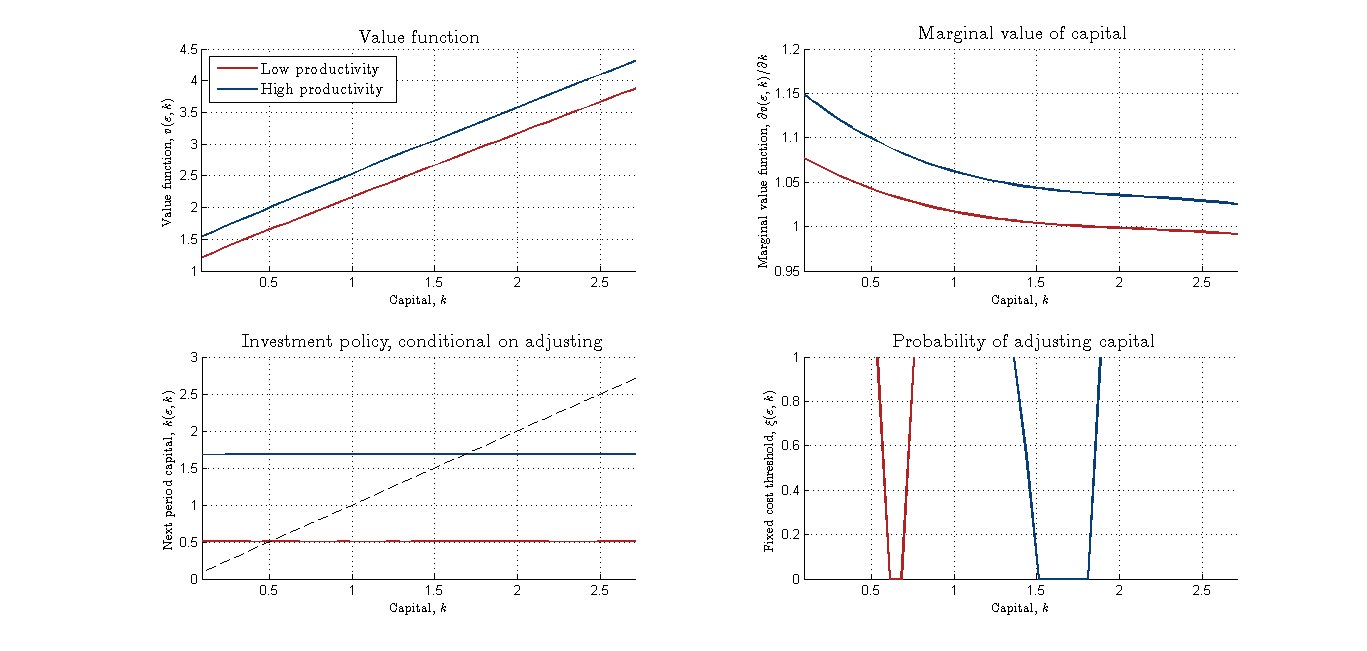
\includegraphics[scale=0.5]{../Appendix/Vf-1.png}
\end{figure}

\begin{figure}[h]
\caption{Tracing investment implications}
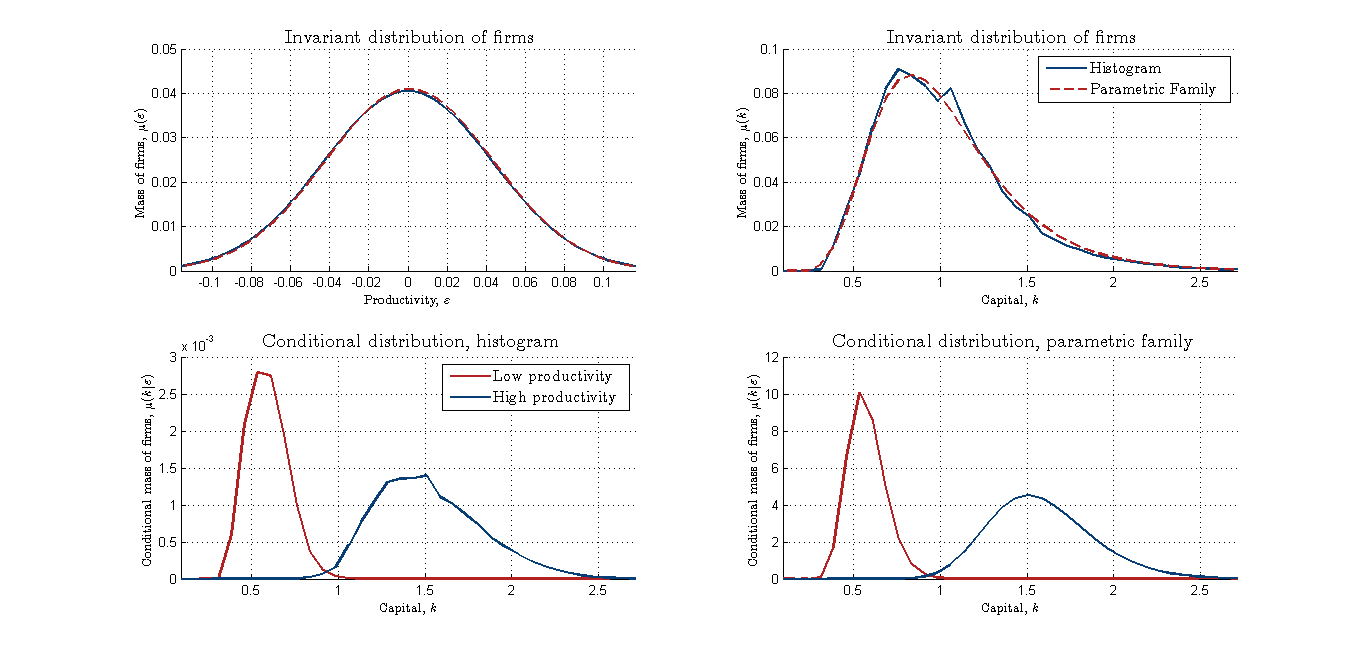
\includegraphics[scale=0.5]{../Appendix/Vf-2.png}
\end{figure}




\end{document}
